\documentclass[12pt]{article}
\usepackage[top=3cm, bottom=3cm, left=2cm, right=2cm]{geometry}
\usepackage{setspace}
\geometry{a4paper} % or letter or a5paper or ... etc
% \geometry{landscape} % rotated page geometry
\usepackage[T1]{fontenc}
\usepackage[applemac]{inputenc}
\usepackage[danish,english]{babel}
\usepackage{amsmath,amssymb,amsthm} % matematik
\usepackage{mathtools}
\usepackage{booktabs} % p�nere tabeller
\usepackage[pdftex]{graphicx}
\usepackage{fancyhdr} % hoved- og sidefod
\usepackage{graphics}
\usepackage{float}
\usepackage{overpic}
\usepackage{graphicx}
\usepackage[table]{xcolor}
\usepackage{tikz}
\usepackage{pgfplots}
\usepackage[normalem]{ulem}
\usepackage{natbib}
\usepackage[justification=centering]{caption}

\usepackage{amssymb} %Creates ���
%\usepackage{amsmath} %Equations and general math, parenthesis included with \eqref
\usepackage{mathtools} %Loads amsmath, includes extensions such as \mathclap, 
\usepackage{pgfplots} %Axis-environment in tikz etc.
\usepackage{tikz} %Graphs, figures etc.
\usepackage{graphicx} %Allows including pictures
\usepackage{geometry} %Makes page formatting easier, [showframe] shows frames on all boxes
\usepackage{floatrow} %Use of \floatfoot to make notes for figures
\usepackage{float} %Makes positioning of images better
\usepackage{booktabs} %Allows use of \cmidrule in tables
\usepackage{tabularx} %Allows \begin{tabularx} which creates better tables
\usepackage{multirow} %Makes it possible to make beautiful footnotes and multirows
\usepackage{array} %Makes it possible to make fixed column width in tables
\usepackage{tabu} %Tables with fixed width, evenly distributed 
\usepackage{fancyhdr} %Allows creating header and footer with \pagestyle{fancy}
\usepackage{wrapfig} %Allows texting around figures, with \begin{wrapfigure}
\usepackage{comment} %Allows using \begin{comment}
\usepackage{sectsty} %Section styles
\usepackage{subfig} %Multiple figures beside each other 
\usepackage{todonotes} %Lav noter og tilh�rende to-do-liste
\usepackage{setspace} %Brug af \begin{spacing} til at angive linjeafstand
\usepackage{fixmath} %G�r math fed med \boldmath
\usepackage[export]{adjustbox} %inner, right, left, osv. ved brug af \includegraphics
\usepackage{chngcntr} % figure numbering, with \counterwithout
\usepackage{etoolbox} %Modify LateX-commands. 







\pagestyle{fancy}
\bibliographystyle{authordate1}
\rhead{Social Data Science}
\lhead{Department of Economics, University of Copenhagen}



\title{}

\numberwithin{equation}{section}
\renewcommand{\baselinestretch}{1.5}
\begin{document}
\input{titlepage}
\pagebreak
\selectlanguage{english}
\tableofcontents
\pagebreak

\section{Introduction / Motivation}
Internet became an important (and continuously expanding) source of information for the Danish citizens in the 21st century. According to the European Commission, Denmark is the European digitalization leader. Almost everyone in the country has at least elementary computer skills and uses internet for a large range of services. People searching any kind of information are primarily looking for it on Google. Over the past three years, Google was Denmark's number one search engine, having a market share of 95 pct\footnote{\url{http://gs.statcounter.com/search-engine-market-share/all/denmark/#monthly-201507-201807}}. Indeed, Google facilitates people's access to information and can contribute to their decision making. 
 
The goal of this paper is to deep the knowledge about the link between the internet searches and the unemployment rate in the Danish labor market (In order to improve the prediction/forecasting of the latter).  

This kind of analysis has been widely discussed by different researchers in the past decade, but to our knowledge, this type of analysis has not been made on the Danish labor market. In the following section we review a few articles that have been investigating the same correlation between Google searches and the unemployment rate.

\section{Literature review}
In their paper "Can Google econometrics predict unemployment? Evidence from Spain" from 2018, Marcos Gonzales-Fernandez and Carmen Gonzales-Velasco find a high correlation between Google searches and the unemployment rate in Spain with monthly data from January 2004 to November 2017. In their analysis they compare a baseline model, a simple AR(1) model, with the model with internet search queries about unemployment, and then with a model with lagged search queries about unemployment. Their results show that the model where search queries are included without any lags is in fact a better model for prediction than their baseline of a simple AR(1), since this model will produce the smallest errors in the prediction of unemployment.

Francesco D'Amuri and Juri Marcucci also find a high predicting power on unemployment in the US from Google searches in their article: "The predictive power of Google searches in forecasting US unemployment" from 2017. They use both a long and short sample size for their predictions, the short sample going from 2004.2 to 2014.2 and long sample going from 1997.7 to 2014.2. Overall, the short sample size seems to be a better predictor compared to the baseline of a basic AR(1) model than the long sample. Their results show that the models using Google search queries achieves the best performance when it comes to root mean squared forecast errors (RMSFEs) with an advantage over the baseline, and it actually increases with the forecast horizon (18 pct. improvement one time step ahead). 

In the literature we find a difference in what the different researchers chooses as search keywords on Google when predicting the unemployment rate. \cite{Fernandez2018} chooses only the word "desempleo", the Spanish word for unemployment, since they assume that this word will summarize the search queries about the situation of loosing a job. Next, other words like payment received when unemployed is in Spanish "subsidio por desempleo", so these queries will already be gathered with the word "desempleo".

\cite{Amuri2017} chooses only the word "jobs" for their queries in their article, since they find this word to be the most popular among different job-search-related keywords. Next, they argue that it is the word that is used most widely across job seekers and thereby is less sensitive to the presence of demand and supply shocks specific to subgroups of workers, which could then bias the value of the GI. Finally, the word "jobs" is not only being used by unemployed people but also employed people, and it thereby captures the overall job-search activity.

Like many other articles within the literature, both \cite{Fernandez2018} and \cite{Amuri2017} gather their internet search data from Google Trends which provides the Google search index (GI). An explanation of this index will follow in the data section below. 


\section{Data}
In this section we present the data for both the Danish unemployment rate and the data used for search queries on Google relating to unemployment.

\subsection{Danish data for unemployment}
There are three different measures for unemployment in Denmark. Gross unemployment, net unemployment and the ILO unemployment survey (AKU arbejdsl\o shedsm\aa let - Arbejdsmarkedsunders\o gelsen). The gross and net are register based measures, and the ILO unemployment survey is a survey measure of unemployed people according to the International Labour Organization. All three measures are published on a monthly basis. 
The gross unemployment rate is defined by registered unemployed in the age from 16 to 64 and whom receive payments from the state or an unemployment insurance fund. The net employed are all registered unemployed who receive payments from an unemployment insurance fund or are marked as "ready for job" but still receive payments from the state. Therefore the gross includes the "activated" and the net does not. Finally the ILO unemployment rate follows the ILO definition of unemployment, i.e. people completely out of a job and are available and are or has been job seeking. Figure \ref{Unemp} plots the three measures both seasonal and non-seasonal on a monthly basis for the period 2007M01 to 2018M06 collected from Statistics Denmark. As Figure \ref{Unemp} shows, the level in the three measures seems to differ whereas the development are approximately the same.

\begin{figure}[h!]
     \caption{Gross-, net- and ILO unemployed, 2007M01 - 2018M06, pct.}
\label{Unemp}
\centering
    \includegraphics [width=1\textwidth] {Figurer/unemp.png} 
    {\footnotesize{Source: Statistics Denmark}}
\end{figure}

We choose to apply the net unemployment rate for our analysis. This is because we would expect that people who are "activated", and thereby included in the gross measure, would not spend as much time doing job related searches on Google. Next, we choose to collect non-seasonal adjusted data, even though unemployment data is highly affected by seasons. This is due to the fact that we need to be consistent in our data selection, and since Google Trends are also non-seasonal adjusted it would be tough to correct these by the same seasonal correction as applied by Statistics Denmark. In the literature, researchers are divided when deciding whether to use seasonal or non-seasonal adjusted data. \cite{Amuri2017} chooses to work with weakly seasonal adjusted unemployment data whereas \cite{Fernandez2018} uses non-seasonal adjusted data. 


In order to apply Machine Learning in this project we need a stationary time series\footnote{\url{https://towardsdatascience.com/how-not-to-use-machine-learning-for-time-series-forecasting-avoiding-the-pitfalls-19f9d7adf424}}. Therefore we choose to drop the first part of our sample, i.e. the data from 2007 to 2010 where we see a big level shift in Figure \ref{Unemp}. We are aware that this will exclude the ability for our model to predict large shocks to unemployment, which is unfortunate. Another way to make the data stationary is to just take the first difference, but in our project with Machine Learning this will not be feasible since the prediction would then always converge towards the mean. With first difference our prediction would therefore always be very close to zero. So we chose our final data sample for net unemployment to be the period from 2010M01 to 2018M06. The data is shown in Figure \ref{Net} below:

\begin{figure}[h!]
     \caption{Net unemployed, non-seasonal adjusted, 2010M01 - 2018M06, pct.}
\label{Net}
\centering
    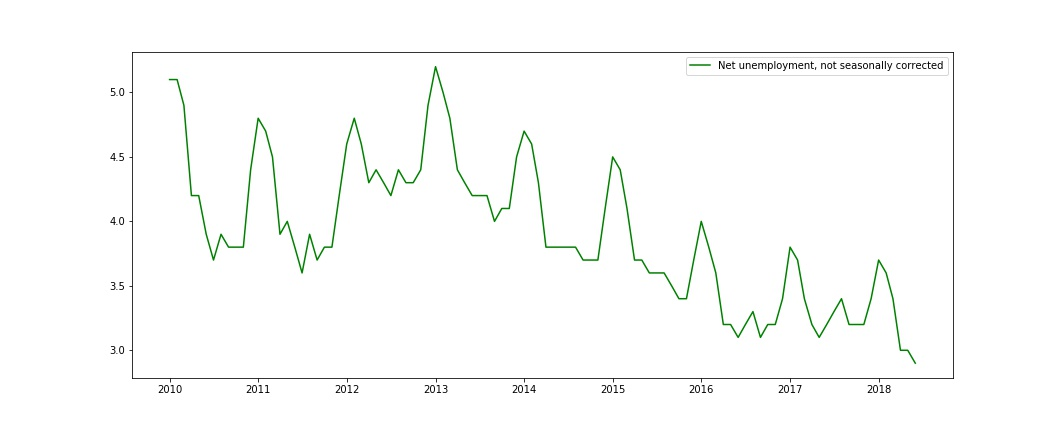
\includegraphics [width=1\textwidth] {Figurer/netunemp.jpg} 
    {\footnotesize{Source: Statistics Denmark}}
\end{figure}

The data of interest is available on www.statistikbanken.dk in Statistics Denmark openly provided statistics "AKU125: Labour Force Status" and "AUS07: Unemployed persons". We pull the data as csv-files from DST's API, using a link constructed through DST's API link console \footnote{\url{https://api.statbank.dk/console}}. The constructed link filters the data of interest:

\begin{itemize}
    \item unemployment in pct. of the total labour force.
    \item for all months 2007-01 to 2018-06.
    \item both seasonally corrected and non-seasonally corrected unemployment rates.
    \item for both ILO-unemployment rate (AKU-arbejdsl\o shed), Gross Unemployment, Net Unemployment.
\end{itemize}



\subsection{The Google Index}
The Google Index (GI) gives the user the possibility to select different search keywords in a given geographical area in a given time frame. From this index, the Search Volume Index, $SVI$, is calculated by the amount of searches on the specific keyword on a specific time and area, $V_t^q$, divided by the total number of searches through Google for the same specific time and area, $V_t$. $SVI_t=\frac{V_t^q}{V_t}$. 
that for privacy and anonymity reasons there is no absolute values for GI components available publicly. Therefore, one can not itself calculate the SVI. But Google helps by scaling the GI to 100 in the week in the chosen sample where it reaches its maximum level. So the GI index represents the likelihood of a random user doing a Google search for the chosen keyword in the specific area and specific time. Finally, it should be mentioned that the index is calculated based on a sample of IPs that changes with time and with the IP address. Therefore, indices can vary according to the specific day, time, and IP used when downloading the data (D'Amuri and Marcucci (2017)). 

We choose to download our GI from Google Trends for the following keywords: "Job", "Kontanthj\ae lp", "A-kasse", "Jobnet"  and "Dagpenge". These words are chosen, since they in our opinion are correlated with the unemployment rate. Next, these keywords should capture all search queries related to unemployment in Denmark. This list can of course be extended/reduced to more or less keywords.

The data from Google Trends consists of time series for each search query keyword. The time interval is set to 2007/01-2018/06 and we only look at Google Trends for searches in Denmark. We enter the keywords on Google Trends \footnote{\url{https://trends.google.com/}} and scrape the associated time series data one by one. The scrape is then performed using GET requests, which returns responses in JSON-format. From the JSON data we extract the data for each keyword and wrangle them into a single combined dataframe.

In Figure \ref{GI} our GIs for our five keywords are shown for the period 2007M01 to 2018M06:

\begin{figure}[h!]
     \caption{Google Index, 2007M01 - 2018M06}
\label{GI}
\centering
    \includegraphics [width=1\textwidth] {Figurer/GIplot.png} 
    {\footnotesize{Source: Google Trends}}
\end{figure}




\section{Method}
In this section we present our method when predicting the unemployment rate in Denmark using Machine Learning.

Since we wish to predict the unemployment rate in the current period, $y_t$, we specify a model that include searches for our keywords in the previous period, $X_{t-1}$, and the unemployment in the previous period, $y_{t-1}$, and finally we add a constant. 
\begin{align}
y_t = k_0 + \beta_i X_{t-1} + \alpha y_{t-1}
\end{align}

\subsection{Linear Regression}
Linear regression is an econometric tool that shows the relationship between the dependent and independent variables using a first-degree function. It has a straight-linear representation tracing the line in a way that minimizes the squared distance between the data and the line. This is a convenient tool when the relationship between the variables is linear.
However, the linear regression takes into account only the mean of the independent variables and can not be used for non-linear relationships. The model is too simple and can not capture enough data. In addition it doesn�t predict a valuable numeric output.
We ran our linear regression model, including all key words and the lagged variable. The results have been used as a benchmark for comparison with the Lasso and Ridge models.

\subsection{Regularization}
A common problem when using machine learning is overfitting of the model. This implies, that model includes features that actually fit the training data too well. The result of overfitting is reduced prediction power, since the model, even though suitable for describing the training data, cannot explain the out-of-sample data, e.g. the test data. 
There exist multiple machine leaning methods that account for overfitting. These are so-called regularization methods, and in this paper we will use two of these, the Least Absolute Shrinkage and Selection Operator (LASSO) and the Ridge regression.



\subsection{Cross-validating time series}
To measure the predictive power of a model, the model should be tested not only on in-sample data but also on out-of-sample data, i.e. cross-validation. In machine learning, popular cross-validation methods are train-test-splits and K-fold. In time series however, data is not independent due to serial correlation, and the aforementioned methods cannot readily be applied.

The train-test-split technique can be altered to time series, by making a split that keeps the order of observations. This is also known as fixed-origin evaluation (\cite{Tashman2000}). For our data, with 101 sequential observations, that means splitting so that the first (e.g. 112) months are used for model development (i.e. training and validation) and the remaining (28) months are used only for testing. A thorough discussion of this and similar techniques can be found in the article by \cite{Tashman2000}. 

A widely used, but simple advancement of the fixed-origin evaulation is the rolling-origin-update evaluation (\cite{Bergmeir2012}). The data is split multiple times at different points. Although the point of the splits varies and the size of the training data thereby varies, the size of the test set always remain the same. That means that some of the most recent data is unused in some of the splits and it therefore also requires a sufficiently long dataset.

The K-fold method is not usable for our data because of the serially correlated nature of time series and the non-stationarity of the unemployment rate. K-folds can however be used for purely autoregressive time series as it has been shown by \cite{Bergmeir2018} but since our proposed prediction model is not purely autoregressive this caveat is not relevant.

\section{Results}

In tabel \ref{Results} we present our results from both the linear regression, the AR(1) mode, the Lasso and the Ridge.

\begin{table}[h!]
\begin{center}
    \caption{Results from predictions using different models and allowing \\ for different degrees of polynomials} 
\begin{tabular}{l c c c c c c c c }
\hline \hline
 Degrees & \multicolumn{2}{c}{Linear} & \multicolumn{2}{c}{AR(1)} & \multicolumn{2}{c}{Lasso} & \multicolumn{2}{c}{Ridge} \\
\cmidrule(lr){2-3} \cmidrule(lr){4-5} \cmidrule(lr){6-7} \cmidrule(lr){8-9} 
   & $MSE$ & $RMSE$ & $MSE$ & $RMSE$ & $MSE$ & $RMSE$ & $MSE$ & $RMSE$ \\
   \hline \\
  1 & 0,051 & 0,226 & 0,037 & 0,193 & 0,024 & 0,154 & 0,024 & 0,154 \\
  2 & - & - & - & - & 0,024 & 0,156 & 0,025 & 0,159\\
  3 & - & - & - & - & 0,027 & 0,166 & 0,031 & 0,175\\
  4 & - & - & - & - & 0,028 & 0,167 & 0,040 & 0,200\\
  %5 & - & - & - & - & 0,028 & 0,169 & 0,050 & 0,223\\
  (...) &  &  &  &  &  &  &  & \\
  %6 & - & - & - & - & 0,028 & 0,169 & 0,069 & 0,263\\
  %7 & - & - & - & - & 0,031 & 0,177 & 0,084 & 0,290\\
  %8 & - & - & - & - & 0,032 & 0,179 & 0,101 & 0,319\\
  %9 & - & - & - & - & 0,032 & 0,180 & 0,121 & 0,348\\
  10 & - & - & - & - & 0,033 & 0,180 & 0,119 & 0,345\\
\hline \hline
\multicolumn{9}{c}{\footnotesize{Note: Degrees indicates the order of polynomials we allow, when the model fit is made.}} \\
\multicolumn{9}{c}{\footnotesize{The MSE and RMSE are the mean-squred errors and root-mean-squared errors between }} \\
\multicolumn{9}{c}{\footnotesize{the prediction of the test sample and the actual values in the test sample.}}
\label{Results}
\end{tabular}
  \end{center}
  \end{table}

\section{Discussion}



\subsection{Decision tree learning}
In this project we have chosen not to use decision tree learning for our model, but as it is often used for Machine Learning, we will briefly explain the idea behind the method and why we chose not to apply it.

The main idea of a decision tree is to break down the data by asking decision based questions to the data. These questions are based on the features of the training set. Of course one should have in mind not to ask to many questions to the data, hence this would result in overfitting the model, i.e. the decision tree gets too deep. After breaking down the data to the best possible fit, the tree learns the series of questions that are asked to the data.
Decision trees are naturally a good tool for classification data, since it is much easier to ask classifying questions to the data. But we are working with time series data in our project, and therefore we would have to create multiple classifiers from our features, i.e. our GI keywords. This would require more work, and is beyond our time frame for this project.


\section{Conclusion}











\cleardoublepage
\bibliography{ref}
\addcontentsline{toc}{section}{\numberline{}References}








\end{document}






